\documentclass[a4paper]{article}

\usepackage[utf8]{inputenc}
\usepackage[spanish]{babel}
\usepackage{graphics}
\usepackage{caption}
\usepackage{subcaption}
\usepackage[demo]{graphicx}
\usepackage{enumitem}
\usepackage{longtable}
\usepackage{listings}
\usepackage{listingsutf8}
\usepackage{framed}
\usepackage{float}
\usepackage{hyperref}
\usepackage{anysize}
\usepackage{fancyhdr}
\usepackage{eurosym}

% para poner encabezado a la derecha
\pagestyle{fancy}
\fancyhf{}
\fancyhead[LE,RO]{Sistemas y Tecnologías Web}

\newcommand{\HRule}{\rule{\linewidth}{0.35mm}} % Defines a new command for the horizontal lines, change thickness here

\begin{document}

% % cambiar margenes
\marginsize{3cm}{3cm}{2.5cm}{2.5cm} 

\begin{flushright}
	\textsc{\huge Práctica 3\\}
	\textsc{\tiny " "\\}
	\textsc{\large
		Jaime Ruiz-Borau Vizárraga (546751)\\
	}
	\HRule \\
\end{flushright}

\section{Diagrama de la base de datos}
\setcounter{page}{1}
\begin{figure}[H]
	\centering
	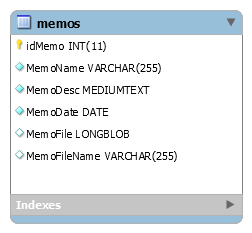
\includegraphics[width=7.5cm,keepaspectratio]{diagramaer}
	\caption{Entidad de la base de datos con sus atributos}
	\label{fig:trayec1ej3}
\end{figure}
\section{Diagrama de dependencias}
\begin{figure}[H]
	\centering
	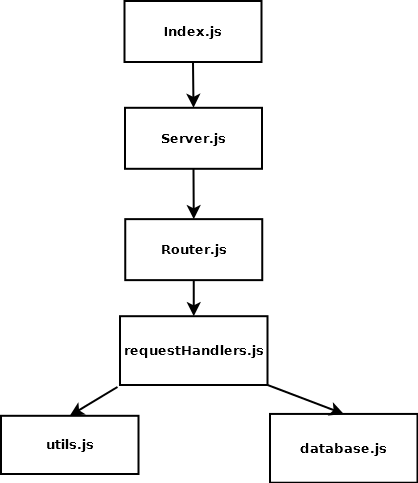
\includegraphics[width=7.5cm,keepaspectratio]{DiagramaJS}
	\caption{Diagrama de dependencias JavaScript}
	\label{fig:trayec1ej3}
\end{figure}


\end{document}